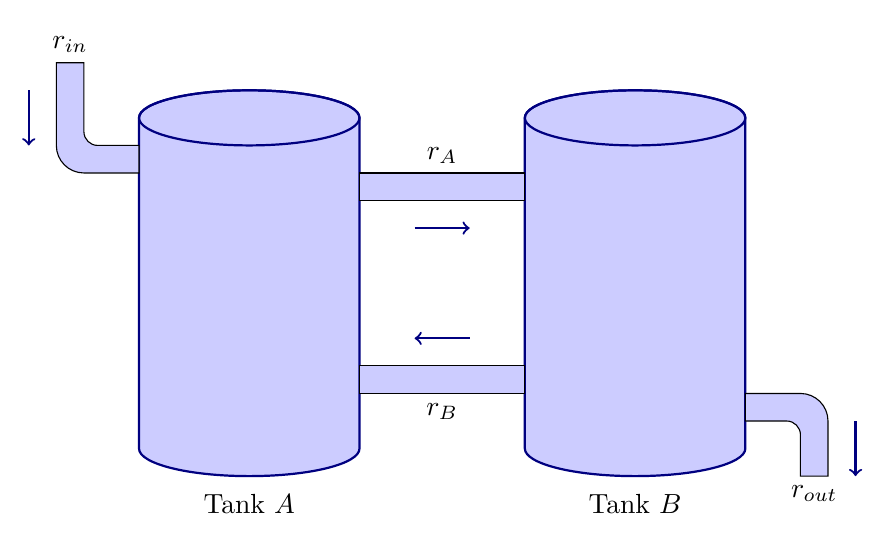
\begin{tikzpicture}[scale=0.7]
\filldraw[fill=blue!20,draw=blue!50!black, thick] (0,0) arc (180:360: 2 and 0.5) -- (4,0) -- (4,6) arc (0:180: 2 and 0.5) -- (0,6) -- cycle;
\draw[blue!50!black, thick] (2,6) ellipse (2 and 0.5);
\filldraw[fill=blue!20,draw=blue!50!black, thick] (7,0) arc (180:360: 2 and 0.5) -- (11,0) -- (11,6) arc (0:180: 2 and 0.5) -- (7,6) -- cycle;
\draw[blue!50!black, thick] (9,6) ellipse (2 and 0.5);
\filldraw[fill=blue!20] (4,1) -- (7,1) -- (7,1.5) -- (4,1.5) -- cycle;
\filldraw[fill=blue!20] (4,4.5) -- (7,4.5) -- (7,5) -- (4,5) -- cycle;
\filldraw[fill=blue!20] (11,1) -- (12,1) arc (90:0:0.5)-- (12.5,-0.5) -- (12,-0.5) -- (12,0.25) arc (0:90:0.25) --  (11,0.5) -- cycle;
\filldraw[fill=blue!20] (-1,7) -- (-1,5.75) arc (180:270:0.25) -- (-0.5,5.5) -- (0,5.5) -- (0,5) -- (-1,5) arc (270:180:0.5) --  (-1.5,7) -- cycle;
\draw[blue!50!black,<-,thick] (5,2) -- (6,2);
\draw[blue!50!black,->,thick] (5,4) -- (6,4);
\draw[blue!50!black,->,thick] (13,0.5) -- (13,-0.5);
\draw[blue!50!black,<-,thick] (-2,5.5) -- (-2,6.5);
\node at (2,-1) {Tank $A$};
\node at (9,-1) {Tank $B$};
\node at (5.5,1) [below] {$r_B$};
\node at (5.5,5) [above] {$r_A$};
\node at (12.25,-0.5) [below] {$r_{\text{out}}$};
\node at (-1.25,7) [above] {$r_{\text{in}}$};
\end{tikzpicture}